\documentclass{beamer}

\usepackage{graphicx}
\usepackage{amssymb}
\usepackage{framed}
\usepackage{subfiles}
\begin{document}
%-------------------------------------------- %
% Schedule 0 
% Leadout
% - PyData Berlin and London
% Schdule 1
%  - Anaconda
%  - Building Bloack - numpy pandas etc
% Schedule 2 
%  - SKL capabilities
%    ======== %
 
 \huge
 
 \[\mbox{Data Science with Python} \]
 { 
 \[\mbox{(with \texttt{scikit.learn}})\]
}
 \bigskip
 \[ \mbox{Big Data Analytics Research Group} \]
 \[ \mbox{University of Limerick} \]
 
%    ======== %
 [fragile]
 \frametitle{Data Science with Python}
  
  
  [(i)] Some Opening Comments
  [(ii)] Python Environment
  [(iii)] What is Machine Learning?
  [(iv)] Useful Packages
  [(iv)] \texttt{scikit.learn}
  
 
 
\subfile{00-leadout.tex}
%        %
 
  \frametitle{Data Science with Python}
 \begin{figure}
  \centering
  \includegraphics[width=1.1\linewidth]{pythonlogo}
  
 \end{figure}
 
 
%        %
 
  \frametitle{Data Science with Python}
  
 \textbf{What is Python?}
 \begin{quote}
  Python is an interpreted, object-oriented, high-level programming language with dynamic semantics. Its high-level built in data structures, combined with dynamic typing and dynamic binding, make it very attractive for Rapid Application Development, as well as for use as a scripting or glue language to connect existing components together. 
 \end{quote}
 
 (Python.org)
 

%        %
 
  \frametitle{Data Science with Python}
  
 \textbf{What is Python?}
 \begin{quote}
  Python's simple, easy to learn syntax emphasizes readability and therefore reduces the cost of program maintenance. Python supports modules and packages, which encourages program modularity and code reuse. The Python interpreter and the extensive standard library are available in source or binary form without charge for all major platforms, and can be freely distributed.
 \end{quote}
 (Python.org)
 
%        % 
 
  \frametitle{Data Science with Python}
  
 \textbf{History of Python}
 \begin{quote}
  Python was created in the early 1990s by Guido van Rossum at Stichting Mathematisch Centrum in the Netherlands as a successor of a language called ABC. Guido remains Python’s principal author, although it includes many contributions from others.
 \end{quote}
 
%      ===== %
 
 \begin{figure}
\centering
\includegraphics[width=1.1\linewidth]{mjasay}

\end{figure}

 
%      ===== %
 
\begin{figure}
\centering
\includegraphics[width=1.1\linewidth]{hypecycle}
\end{figure}
 
 
 \begin{figure}
\centering
\includegraphics[width=0.9\linewidth]{mjasay2}
\end{figure}

 
%      ===== %
 
 \begin{figure}
\centering
\includegraphics[width=1.1\linewidth]{KnowledgePyramid}
\end{figure}
 

%      ===== %
\subfile{01-Introduction.tex}
\subfile{01-versionsconventions.tex}
%    ======== % 
\subfile{02-machinelearning}
\subfile{02-visualization.tex}


%\subfile{02-packages.tex}
%     ======== %
 
 \huge
 Three Core Packages
 \begin{enumerate}
   numpy
   pandas
   scipy
 \end{enumerate}
 \begin{figure}
\centering
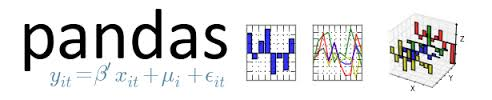
\includegraphics[width=0.7\linewidth]{pandaslogo}\\
\includegraphics[width=0.7\linewidth]{scipylogo}

\end{figure}

 
%       %
\subfile{numpy.tex}
\subfile{pandas}
\subfile{scipy.tex}
%      ===== %
 
 \begin{figure}
  \centering
  \includegraphics[width=1.1\linewidth]{machinelearningquotes}
 \end{figure}
   Machine Learning is Statistics minus any checking of models or assumptions
 
%   =%
 
 \frametitle{The Data Science Profession}
 Data Science Retreat (Berlin)
 \begin{quote}
  MOOC have not  decreased the barrier of entry to machine-learning.
  
  
  
  Nowadays, you cannot be 'the guy who knows how to run (insert off-the-shelf-algo-here)'. 
  
  
  In dataland, that's the equivalent to being a code monkey. MOOCs and superb libraries (scikit-learn, R's ecosystem) made 
  sure there is plenty of people who can throw say a random forest to a problem. In the modern world, this is not adding that much value. 
 \end{quote}
 
%      =====%

 
 \frametitle{scikit.learn}
 \begin{figure}
  \centering
  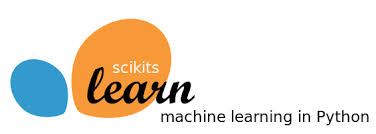
\includegraphics[width=0.5\linewidth]{SKL-logo2}
  
 \end{figure}
 
  
   scikit-learn is an open source machine learning library for the Python programming language. 
   scikit-learn features various classification, regression and clustering algorithms including support vector machines, logistic regression, naive Bayes, random forests, gradient boosting, k-means and DBSCAN.  scikit-learn is designed to interoperate with the Python numerical and scientific libraries NumPy and SciPy.
  
 
%      =====%
 
 \textbf{Sci-Kit Learn Site info}
 \begin{figure}
  \centering
  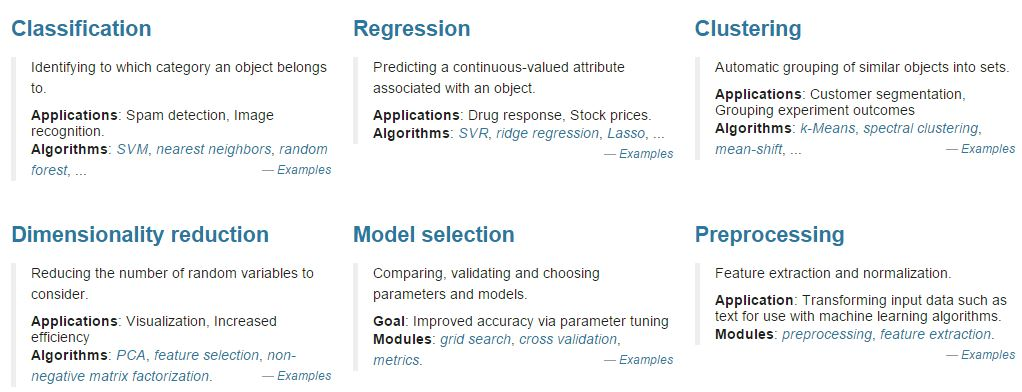
\includegraphics[width=1.1\linewidth]{SKLsiteinfo}
 \end{figure}
 
%      =====%
 
 \begin{figure}
  \centering
  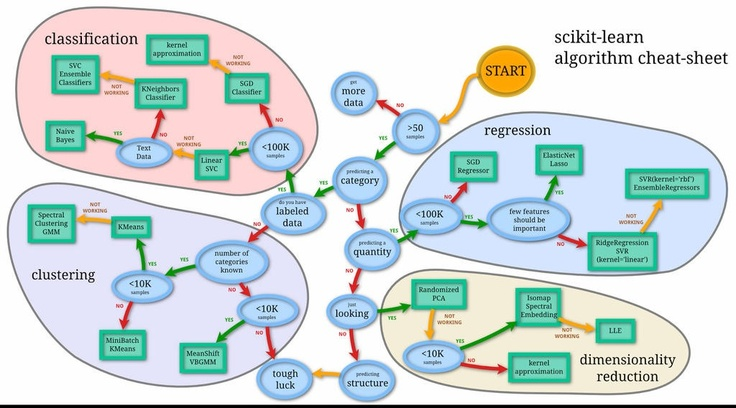
\includegraphics[width=0.9\linewidth]{SKLCheatSheet}
  
 \end{figure}
 
%      =====%
 
 \begin{figure}
  \centering
  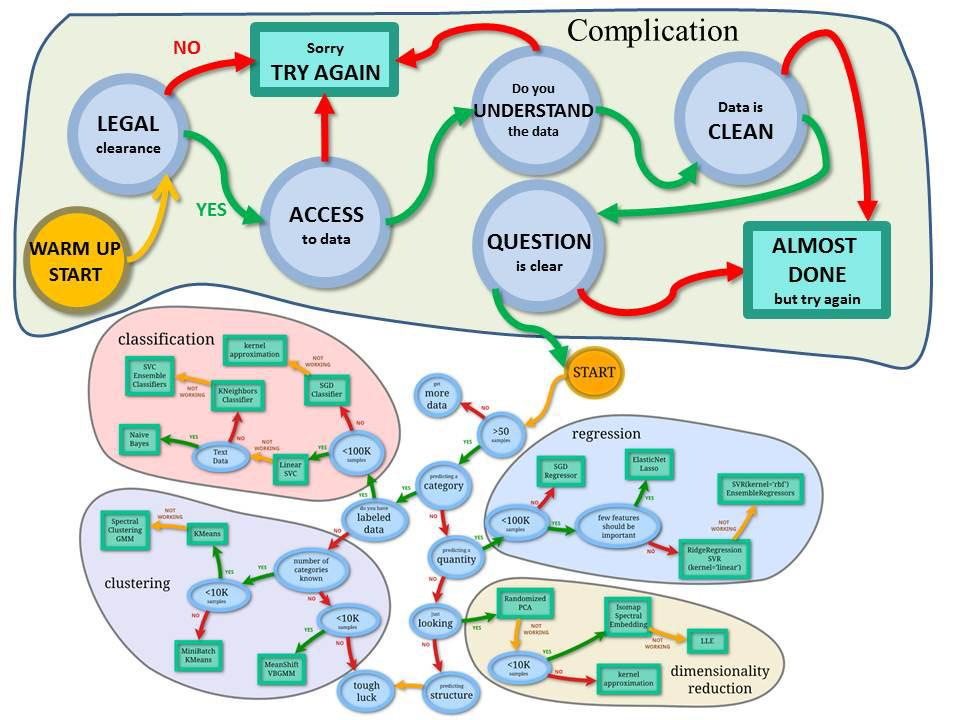
\includegraphics[width=0.9\linewidth]{SKLCheatSheet2}
  
 \end{figure}
 

\subfile{02-skltopics.tex}
%\subfile{01-Introduction.tex}


%      =====%
 
 \frametitle{statsmodels}
  
 \textbf{statsmodel}
  
   \texttt{statsmodels} provides a large range of cross-sectional models aswell assometime-series models. 
   statsmodels
  uses a model descriptive language (provided via the Python package patsy) to formulate the model
  when working with pandas \texttt{DataFrames}.
   Models supported include linear regression, generalized linear
  models, limited dependent variable models, ARMA and VAR models.
  
 
\subfile{textmining.tex}
%\subfile{03-datastructures.tex}
%\subfile{06-specialarrays.tex}

%\subfile{09-probdistributions.tex}
\subfile{07-sklclass.tex}
\subfile{03-decisiontrees.tex}
\subfile{03-SVMs.tex}


%    ======== % 


\end{document}
